% !TEX program = pdflatex
% Slide Beamer. Mọi con số lấy từ ../../report/generated (do chương trình sinh ra), không gõ tay.
\documentclass[aspectratio=169,10pt,t]{beamer}
\usepackage{lmodern}          % Computer Modern (Latin Modern); nạp trước fontenc để T5 dùng t5-lmr
\renewcommand{\sfdefault}{\rmdefault}      % mọi chữ là Computer Modern có chân
\renewcommand{\familydefault}{\rmdefault}
\usepackage[T5]{fontenc}
\usepackage[utf8]{inputenc}
\usepackage{microtype}
\usepackage{amsmath,amssymb,bm}
\usepackage{booktabs,array}
\usepackage{graphicx}
\usepackage{xurl}
\graphicspath{{../../results/figures/}{./}}

% Giao diện Beamer trung tính: nền trắng, chữ Computer Modern có chân, một màu nhấn xanh navy
\usetheme{default}
\usefonttheme{serif}           % phải đặt sau \usetheme, nếu không theme mặc định đổi về phông không chân
\definecolor{navy}{HTML}{1F3A5F}
\setbeamercolor{structure}{fg=navy}
\setbeamercolor{frametitle}{fg=navy,bg=white}
\setbeamercolor{block title}{fg=navy,bg=navy!10}
\setbeamercolor{block body}{fg=black,bg=navy!4}
\setbeamerfont{frametitle}{size=\large,series=\bfseries}
\setbeamertemplate{navigation symbols}{}
\setbeamertemplate{itemize item}{\small\raise0.2ex\hbox{$\blacktriangleright$}}
\setbeamertemplate{frametitle}{\vskip1ex\insertframetitle\par\vskip0.6ex{\color{navy}\hrule height 0.5pt}}
\setbeamertemplate{footline}{\vskip-2pt{\color{navy}\hrule height 0.4pt}\vskip3pt
  \hbox to\paperwidth{\hspace{1.2em}\scriptsize\color{black!70}Trần Trinh Nhân, Lâm Nhật Tiến\hfill Nhận dạng chữ số MNIST\hfill\insertframenumber\,/\,\inserttotalframenumber\hspace{1.2em}}\vskip4pt}
\providecommand{\R}{\mathbb{R}}
% generated by src/experiments/texfrag.py -- do not edit
\newcommand{\accTrainNB}{80.13}
\newcommand{\accValNB}{79.67}
\newcommand{\accTestNB}{81.32}
\newcommand{\foneNB}{81.16}
\newcommand{\precNB}{82.98}
\newcommand{\recNB}{80.95}
\newcommand{\errorsNB}{1868}
\newcommand{\fitNB}{0.4}
\newcommand{\predNB}{0.226}
\newcommand{\latNB}{0.076}
\newcommand{\gapNB}{-1.19}
\newcommand{\accTestSkNB}{81.32}
\newcommand{\fitSkNB}{0.2}
\newcommand{\diffSkNB}{0.00}
\newcommand{\ntrialsNB}{12}
\newcommand{\bestValNB}{79.67}
\newcommand{\accTrainSM}{93.62}
\newcommand{\accValSM}{92.15}
\newcommand{\accTestSM}{92.52}
\newcommand{\foneSM}{92.42}
\newcommand{\precSM}{92.45}
\newcommand{\recSM}{92.41}
\newcommand{\errorsSM}{748}
\newcommand{\fitSM}{12.7}
\newcommand{\predSM}{0.024}
\newcommand{\latSM}{0.010}
\newcommand{\gapSM}{1.10}
\newcommand{\accTestSkSM}{91.86}
\newcommand{\fitSkSM}{154.6}
\newcommand{\diffSkSM}{0.66}
\newcommand{\ntrialsSM}{16}
\newcommand{\bestValSM}{92.15}
\newcommand{\accTrainMLP}{99.87}
\newcommand{\accValMLP}{98.18}
\newcommand{\accTestMLP}{98.24}
\newcommand{\foneMLP}{98.23}
\newcommand{\precMLP}{98.23}
\newcommand{\recMLP}{98.23}
\newcommand{\errorsMLP}{176}
\newcommand{\fitMLP}{11.0}
\newcommand{\predMLP}{0.051}
\newcommand{\latMLP}{0.042}
\newcommand{\gapMLP}{1.63}
\newcommand{\accTestSkMLP}{98.02}
\newcommand{\fitSkMLP}{57.8}
\newcommand{\diffSkMLP}{0.22}
\newcommand{\ntrialsMLP}{22}
\newcommand{\bestValMLP}{98.18}
\newcommand{\accTrainADA}{100.00}
\newcommand{\accValADA}{97.59}
\newcommand{\accTestADA}{97.60}
\newcommand{\foneADA}{97.58}
\newcommand{\precADA}{97.58}
\newcommand{\recADA}{97.58}
\newcommand{\errorsADA}{240}
\newcommand{\fitADA}{817.9}
\newcommand{\predADA}{0.751}
\newcommand{\latADA}{18.705}
\newcommand{\gapADA}{2.40}
\newcommand{\accTestSkADA}{97.50}
\newcommand{\fitSkADA}{1892.8}
\newcommand{\diffSkADA}{0.10}
\newcommand{\ntrialsADA}{14}
\newcommand{\bestValADA}{97.59}
\newcommand{\accTrainCNN}{99.40}
\newcommand{\accValCNN}{98.65}
\newcommand{\accTestCNN}{98.80}
\newcommand{\foneCNN}{98.79}
\newcommand{\precCNN}{98.79}
\newcommand{\recCNN}{98.79}
\newcommand{\errorsCNN}{120}
\newcommand{\fitCNN}{143.0}
\newcommand{\predCNN}{1.163}
\newcommand{\latCNN}{0.315}
\newcommand{\gapCNN}{0.60}
\newcommand{\ntrialsCNN}{10}
\newcommand{\bestValCNN}{98.65}
\newcommand{\splitFingerprint}{52cc8206ff96f56d}
\newcommand{\pixMean}{0.1306}
\newcommand{\pixStd}{0.3081}

% generated by src/experiments/extras_report.py -- do not edit
\newcommand{\crossNB}{49.80}
\newcommand{\ownEmnistNB}{80.03}
\newcommand{\crossSM}{53.59}
\newcommand{\ownEmnistSM}{93.81}
\newcommand{\crossMLP}{76.70}
\newcommand{\ownEmnistMLP}{98.36}
\newcommand{\crossCNN}{92.15}
\newcommand{\ownEmnistCNN}{98.64}
\newcommand{\crossADA}{73.69}
\newcommand{\ownEmnistADA}{97.38}

\newcommand{\fig}[2][\linewidth]{\includegraphics[width=#1]{#2}}
\newcommand{\maybefig}[2][\linewidth]{\IfFileExists{../../results/figures/#2.png}{\includegraphics[width=#1]{#2.png}}{\emph{(hình chưa được sinh)}}}

\title{Nhận dạng chữ số viết tay MNIST}
\subtitle{Bốn bộ phân lớp tự cài đặt, một mạng tích chập nhỏ, đo trên cùng một giao thức}
\author{Trần Trinh Nhân (24280088) \and Lâm Nhật Tiến (24280029)}
\date{Nhận dạng mẫu -- Đồ án giữa kỳ}

\begin{document}

\begin{frame}[plain]
  \vfill\centering
  {\Large\bfseries\color{navy} Nhận dạng chữ số viết tay MNIST}\par\medskip
  {\normalsize Bốn bộ phân lớp tự cài đặt, một mạng tích chập nhỏ,\\đo trên cùng một giao thức và đối chiếu với scikit-learn}\par\bigskip
  {\color{navy}\hrule height 0.5pt}\bigskip
  Trần Trinh Nhân (24280088) \quad Lâm Nhật Tiến (24280029)\par\smallskip
  {\small Nhận dạng mẫu -- Đồ án giữa kỳ}
  \vfill
\end{frame}

\begin{frame}{Đọc một chữ số $28\times28$ và trả lời nó là số nào}
  \begin{columns}[T]
    \column{0.5\linewidth}
    \begin{itemize}\setlength{\itemsep}{6pt}
      \item MNIST: 60\,000 ảnh huấn luyện, 10\,000 ảnh test, 10 lớp; mỗi ảnh có 784 pixel xám.
      \item Câu hỏi: các họ phương pháp khác nhau cho kết quả ra sao khi cùng làm một bài và cùng đo một cách?
      \item Mở rộng: Fashion-MNIST, EMNIST Digits, tăng cường dữ liệu, một CNN nhỏ và một trình khám phá quá trình tính toán trong trình duyệt.
    \end{itemize}
    \column{0.48\linewidth}
    \fig{eda_overview.png}
  \end{columns}
\end{frame}

\begin{frame}{Giao thức: không rò rỉ dữ liệu, chạy lại được bằng một lệnh}
  \begin{columns}[T]
    \column{0.5\linewidth}
    \begin{block}{Ba tập, ba vai}
      Train để học, validation để chọn, test để báo cáo. Hàm tìm siêu tham số không nhận tập test; một kiểm thử tự động giữ điều đó.
    \end{block}
    \begin{block}{Chuẩn hóa chỉ từ train}
      Trung bình và độ lệch chuẩn tính trên 50\,000 ảnh train, dùng lại nguyên si cho validation, test và trình duyệt.
    \end{block}
    \column{0.46\linewidth}
    \small\ttfamily
    prepare $\to$ chia 50\,000/10\,000\\
    tune $\to$ chọn trên validation\\
    train $\to$ huấn luyện lại\\
    evaluate $\to$ test, một lần\\
    export $\to$ ONNX + kiểm tra số\\
    report $\to$ bảng, hình
  \end{columns}
\end{frame}

\begin{frame}{Năm mô hình, năm cách nhìn khác nhau về chữ số}
  \small
  \begin{tabular}{@{}p{4.1cm}p{8.8cm}@{}}
    \toprule
    \textbf{Gaussian Naïve Bayes} & mỗi pixel là một phân phối chuẩn riêng theo lớp, các pixel độc lập \\
    \textbf{Hồi quy softmax} & một mẫu $\bm{w}_k$ cho mỗi lớp, học bằng gradient descent trên cross-entropy \\
    \textbf{MLP} & hai lớp ẩn ReLU, lan truyền ngược viết tay, momentum, dừng sớm \\
    \textbf{AdaBoost-SAMME} & hàng trăm cây quyết định có trọng số; cây sau tập trung vào ảnh cây trước làm sai \\
    \textbf{CNN nhỏ} & hai khối tích chập + max-pool + ReLU, rồi lớp dày đặc; im2col và gradient viết tay \\
    \bottomrule
  \end{tabular}
\end{frame}

\begin{frame}{Phần lõi tự viết, thư viện chỉ để kiểm tra}
  \begin{columns}[T]
    \column{0.55\linewidth}
    \begin{itemize}\setlength{\itemsep}{5pt}
      \item Ước lượng tham số, loss, gradient và cập nhật viết tay bằng NumPy; MLP và CNN dùng PyTorch \emph{chỉ làm kho tensor}: không autograd, không \texttt{nn.Module}, không \texttt{optim}, không \texttt{F.conv2d}, không \texttt{F.max\_pool2d}.
      \item scikit-learn chỉ để đối chiếu.
    \end{itemize}
    \column{0.42\linewidth}
    \begin{block}{121%
 kiểm thử tự động}
      Gradient giải tích khớp sai phân hữu hạn; backprop và gradient CNN khớp autograd; convolution khớp vòng lặp ngây thơ; cây có trọng số khớp \texttt{DecisionTreeClassifier}.
    \end{block}
  \end{columns}
\end{frame}

\begin{frame}{Chọn siêu tham số: quét từng tham số một, chọn bằng validation}
  \begin{columns}[T]
    \column{0.5\linewidth}
    \fig{sweep_mlp.png}
    \column{0.48\linewidth}
    \small
    \begin{itemize}\setlength{\itemsep}{4pt}
      \item Công cụ: \textbf{tự viết}, không dùng Optuna. Mỗi tham số được quét riêng theo từng bước (coordinate descent), chi phí là tổng số giá trị thay vì tích.
      \item Chọn theo accuracy trên validation; mọi lần chạy được ghi lại bằng Weights \& Biases.
      \item Đồ thị trái chính là hình ``đổi một siêu tham số, giữ nguyên phần còn lại'' mà đề bài yêu cầu.
      \item Giới hạn: không xét tương tác giữa các siêu tham số.
    \end{itemize}
  \end{columns}
\end{frame}

\begin{frame}{Kết quả trên tập test}
  \begin{columns}[T]
    \column{0.45\linewidth}
    \small
    \begin{tabular}{@{}lr@{}}
      \toprule
      Mô hình & Test accuracy \\
      \midrule
      Gaussian NB & \accTestNB\,\% \\
      Softmax & \accTestSM\,\% \\
      MLP & \accTestMLP\,\% \\
      AdaBoost-SAMME & \accTestADA\,\% \\
      CNN nhỏ & \accTestCNN\,\% \\
      \bottomrule
    \end{tabular}\par\medskip
    \footnotesize Một seed (42), 10\,000 ảnh test. Khoảng tin cậy 95\% mỗi số rộng cỡ $\pm0.3$ điểm; so sánh cặp bằng kiểm định McNemar chính xác.
    \column{0.52\linewidth}
    \fig{benchmark.png}
  \end{columns}
\end{frame}

\begin{frame}{Độ chính xác không đi cùng thời gian}
  \small
  \begin{tabular}{@{}lrrr@{}}
    \toprule
    Mô hình & Test (\%) & Huấn luyện (s) & Một ảnh (ms) \\
    \midrule
    Gaussian NB & \accTestNB & \fitNB & \latNB \\
    Softmax & \accTestSM & \fitSM & \latSM \\
    MLP & \accTestMLP & \fitMLP & \latMLP \\
    AdaBoost-SAMME & \accTestADA & \fitADA & \latADA \\
    CNN nhỏ & \accTestCNN & \fitCNN & \latCNN \\
    \bottomrule
  \end{tabular}\par\medskip
  \footnotesize Toàn bộ trên CPU (không dùng GPU): các phép tính dùng BLAS đa luồng của NumPy/PyTorch; GPU không dùng vì bản PyTorch cài là bản CPU. AdaBoost duyệt hàng trăm cây cho mỗi ảnh nên chậm nhất.
\end{frame}

\begin{frame}{Lỗi tập trung ở các cặp có nét giống nhau}
  \centering\fig[0.82\linewidth]{confusion_all.png}
\end{frame}

\begin{frame}{Cùng siêu tham số, kết quả sát scikit-learn}
  \small
  \begin{tabular}{@{}lrrr@{}}
    \toprule
    Mô hình & Bản của nhóm & scikit-learn & Chênh \\
    \midrule
    Gaussian NB & \accTestNB & \accTestSkNB & \diffSkNB \\
    Softmax & \accTestSM & \accTestSkSM & \diffSkSM \\
    MLP & \accTestMLP & \accTestSkMLP & \diffSkMLP \\
    AdaBoost-SAMME & \accTestADA & \accTestSkADA & \diffSkADA \\
    \bottomrule
  \end{tabular}\par\medskip
  \footnotesize Softmax chênh vì L-BFGS của scikit-learn chạm giới hạn vòng lặp, không dừng sớm như bản của nhóm. Thời gian AdaBoost không so trực tiếp được vì hai bên chia ngưỡng khác nhau.
\end{frame}

\begin{frame}{Mô hình học được gì: có cái đọc được bằng mắt, có cái thì không}
  \centering\fig[0.78\linewidth]{interpretability.png}
\end{frame}

\begin{frame}{Mở rộng 1: Fashion-MNIST và EMNIST Digits}
  \begin{columns}[T]
    \column{0.5\linewidth}
    \begin{itemize}\setlength{\itemsep}{5pt}
      \item Cùng mã, cùng giao thức, cùng bộ đánh giá; chia train/val/test riêng cho từng tập và báo cáo tách biệt.
      \item Tên lớp khác nhau (áo, giày\ldots{} so với chữ số), nên mô hình huấn luyện trên một tập \emph{không} được đánh giá trên tập khác nếu định nghĩa lớp khác nhau; chương trình từ chối phép đó.
      \item Chỉ có một phép kiểm tra chéo hợp lệ: MNIST $\to$ EMNIST Digits (cùng 10 chữ số), báo cáo riêng cho mô hình huấn luyện trên MNIST: Naïve Bayes \crossNB\,\% (so với \ownEmnistNB\,\% khi huấn luyện trên EMNIST), CNN \crossCNN\,\% (so với \ownEmnistCNN\,\%).
    \end{itemize}
    \column{0.48\linewidth}
    \fig{datasets_accuracy.png}\par\smallskip
    {\footnotesize Siêu tham số của Fashion-MNIST và EMNIST Digits chọn bằng quét rút gọn một seed; chênh lệch nhỏ giữa MLP và CNN ở đó chưa đủ để kết luận.}
  \end{columns}
\end{frame}

\begin{frame}{Mở rộng 2: tăng cường dữ liệu, thí nghiệm có đối chứng}
  \begin{columns}[T]
    \column{0.4\linewidth}
    \small
    \begin{itemize}\setlength{\itemsep}{4pt}
      \item Năm phép: xoay, dịch, co giãn, nhiễu Gauss, nhiễu muối tiêu; chỉ tác động lên tập train.
      \item Điều kiện: gốc, từng phép riêng lẻ, nhóm hình học, cả năm; nhiều seed ghép cặp.
      \item Chọn điều kiện \emph{chỉ} theo validation; test dùng để báo cáo và đo độ bền với nhiễu mạnh hơn lúc huấn luyện.
    \end{itemize}
    \column{0.58\linewidth}
    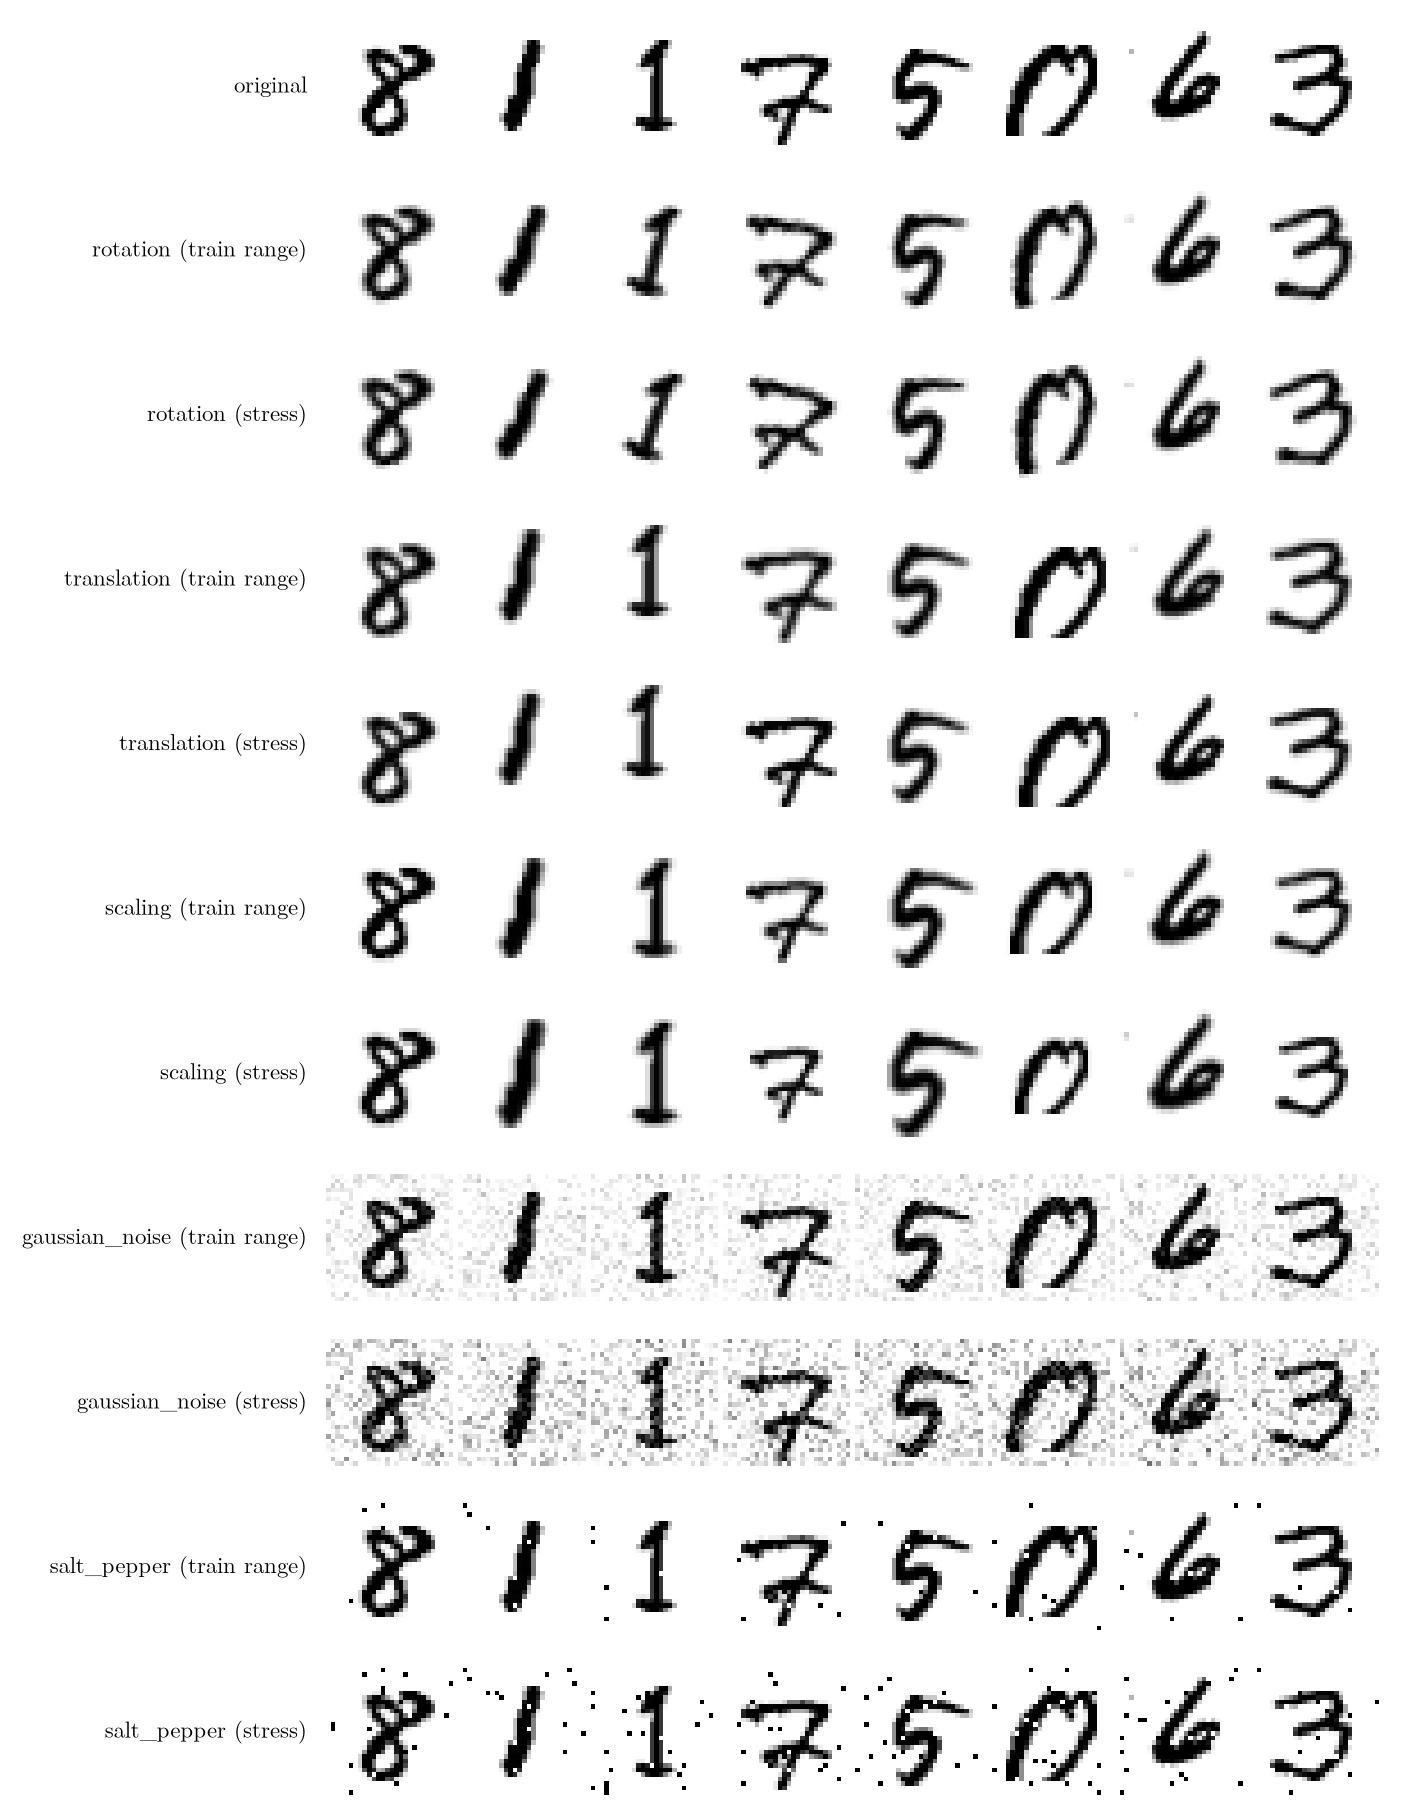
\includegraphics[height=0.78\textheight,keepaspectratio]{augmentation_examples.png}
  \end{columns}
\end{frame}

\begin{frame}{Tăng cường dữ liệu: phép nào giúp, phép nào hại}
  \centering
  \fig[0.93\linewidth]{augmentation_mlp.png}\par\smallskip
  \footnotesize MLP, 3 seed. Mọi phép cho validation cao hơn gốc nhưng cùng bậc với độ lệch chuẩn của hiệu ghép cặp; tác dụng rõ nhất là độ bền với \emph{đúng loại} biến đổi (ví dụ dịch). ``Cả năm phép'' không hơn các phép riêng lẻ.
\end{frame}

\begin{frame}{Tăng cường dữ liệu cho CNN: có phép làm giảm độ bền}
  \centering
  \fig[0.93\linewidth]{augmentation_cnn.png}\par\smallskip
  \footnotesize CNN, 2 seed (độ lệch chuẩn kém tin cậy). Cả năm phép được chọn theo validation. Chỉ dịch hoặc nhóm hình học làm CNN kém bền hơn với nhiễu Gauss và muối tiêu. Mỗi điều kiện có dữ liệu gấp đôi nên loại biến đổi và lượng dữ liệu bị trộn lẫn.
\end{frame}

\begin{frame}{Mở rộng 3: CNN nhỏ so với MLP}
  \centering
  \IfFileExists{../../results/figures/cnn_vs_mlp.png}{\fig[0.95\linewidth]{cnn_vs_mlp.png}}{\emph{Hình so sánh CNN và MLP được sinh sau khi hoàn tất thí nghiệm.}}\par\smallskip
  \footnotesize CNN: \accTestCNN\,\% so với MLP \accTestMLP\,\%. Kích thước, kênh, kernel và lớp dày đặc đều lấy từ \texttt{CNN.describe()} của mô hình thật; mọi tham số đã quét được ghi lại.
\end{frame}

\begin{frame}{Trình khám phá quá trình tính toán chạy trong trình duyệt}
  \begin{columns}[T]
    \column{0.5\linewidth}
    \small
    \begin{itemize}\setlength{\itemsep}{4pt}
      \item Python sinh một \emph{hợp đồng vết} (\texttt{writerhand.trace/1}) từ chính mô hình đã huấn luyện: đồ thị lớp, hình dạng tensor, tiền xử lý, tham số, mã băm.
      \item Trình duyệt chạy ONNX Runtime Web trên ảnh vừa vẽ và vẽ sơ đồ \emph{từ metadata}, không có kiến trúc nào được gõ cứng; đổi mô hình hay ảnh thì kết quả cũ bị loại.
      \item Mỗi phép tính trung gian được tái dựng từ tham số và đối chiếu với giá trị ONNX.
    \end{itemize}
    \column{0.48\linewidth}
    \fig{explorer_crop.png}
  \end{columns}
\end{frame}

\begin{frame}{Trực quan hóa tính toán không phải là giải thích quyết định}
  \begin{block}{Phân biệt}
    Bản đồ kích hoạt của một lớp cho thấy lớp đó \emph{tính ra gì} với ảnh này; nó không chứng minh pixel hay bộ lọc nào \emph{gây ra} quyết định. Với softmax và Naïve Bayes, phân rã $x_iW_{ik}$ hay log-likelihood theo pixel là chính xác (mô hình tuyến tính/cộng tính), và được ghi nhãn như vậy.
  \end{block}
  \begin{block}{AdaBoost}
    Các con số cộng dồn là \emph{tỉ lệ phiếu có trọng số}, không phải xác suất đã hiệu chỉnh.
  \end{block}
\end{frame}

\begin{frame}{Kết luận}
  \begin{columns}[T]
    \column{0.5\linewidth}
    \textbf{Điều rút ra}
    \begin{itemize}\setlength{\itemsep}{4pt}
      \item CNN cho kết quả tốt nhất trên MNIST và EMNIST Digits (khoảng một phần mười số tham số của MLP); trên Fashion-MNIST CNN và MLP ngang nhau.
      \item AdaBoost sát nhưng đắt gấp hàng chục lần khi suy luận.
      \item Chọn cấu hình có kỷ luật quan trọng ngang chọn thuật toán.
    \end{itemize}
    \column{0.46\linewidth}
    \textbf{Giới hạn}
    \begin{itemize}\setlength{\itemsep}{4pt}
      \item Một seed cho các mô hình chính.
      \item Quét tuần tự chưa xét tương tác siêu tham số.
      \item Thời gian đo trên một máy CPU.
      \item Kết quả chỉ nói về các tập đã đo, không phải chữ viết tay nói chung.
    \end{itemize}
  \end{columns}
\end{frame}

\begin{frame}{Đóng góp, công bố sử dụng AI, liên kết}
  \small
  \begin{itemize}\setlength{\itemsep}{5pt}
    \item Đóng góp 50\,\%/50\,\% (Trần Trinh Nhân, Lâm Nhật Tiến), do hai thành viên thống nhất.
    \item Phần hoàn thiện sau commit \texttt{f9a602b} được viết với sự hỗ trợ của Claude Code; số liệu trong báo cáo, bảng và slide đều sinh từ tệp kết quả do chương trình ghi ra.
    \item Mã nguồn: \url{https://github.com/TranTrinhNhan1/WriteRHand}
    \item Demo: \url{https://trantrinhnhan1.github.io/WriteRHand/}
    \item Mô hình: \url{https://huggingface.co/TranTrinhNhan1111/WriteRHand-MNIST}
  \end{itemize}
  \vfill\centering\large Cảm ơn thầy cô và các bạn đã lắng nghe.
\end{frame}
\end{document}
